%!tikz editor 1.0
\documentclass[tikz]{standalone}


%!tikz preamble begin
\usepackage{tikz}
\usetikzlibrary{arrows,positioning,fit}
\usetikzlibrary{overlay-beamer-styles}

\xdefinecolor{color1}{rgb}{1.0, 0, 0}
\xdefinecolor{color2}{rgb}{0, 0.5, 1.0}

\tikzset{
    p1/.style={circle, draw, thick, minimum size=6mm, inner sep=0},
    p2/.style={rectangle, draw, thick, minimum size=5mm, inner sep=0},
    pre/.style = {<-, semithick, >=stealth', shorten <=1pt},
    post/.style= {->, semithick, >=stealth', shorten >=1pt},
  }
%!tikz preamble end


\begin{document}
%!tikz source begin
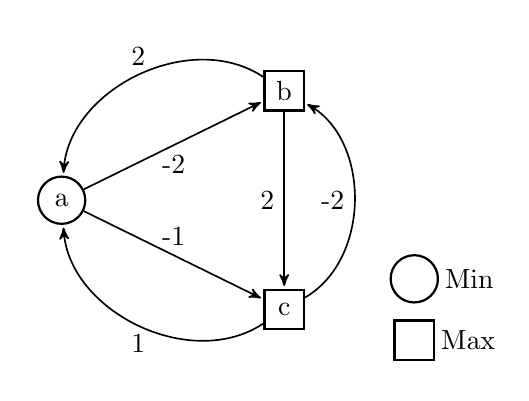
\begin{tikzpicture}
      \node (origin) at (0,0) {};
      \node (a) [p1, left=of origin] {a};
	  \node (b) [p2, above right=of origin] {b};
	  \node (c) [p2, below right=of origin] {c};
        	
	  \draw[->]	(a) edge [post] node [below] {-2} (b)
				(a) edge [post] node [above] {-1} (c)
				(b) edge [post] node [left] {2} (c)
				(c) edge [post, bend right=60] node[left] {-2} (b)
				(c) edge [post, bend left=60] node [below] {1} (a)
				(b) edge [post, bend right=60] node [above] {2} (a);
;

			
  	  \node (graph) [fit=(a) (b) (c)] {};
      \begin{scope}[inner sep=2pt, minimum size=1pt]
        \node (odd-sym) [p2, right=of graph.south east , label={right:Max}] {};
    		\node [p1, above=2mm of odd-sym, label={right:Min}] {};
      \end{scope}
  \end{tikzpicture}
%!tikz source end

\end{document}